% KDD-style manuscript entry point for the BISON course-project paper.
% Author: fangtoast
% Email: fangtoast@foxmail.com
% Copyright (c) 2026 fangtoast. All rights reserved.

\documentclass[sigconf]{acmart}

\setcopyright{none}
\settopmatter{printfolios=true}
\renewcommand\footnotetextcopyrightpermission[1]{}

\usepackage{amsmath}
\usepackage{booktabs}
\usepackage{graphicx}
\usepackage{mathtools}
\usepackage{multirow}
\usepackage{tikz}
\usepackage{xcolor}
\usetikzlibrary{arrows.meta,fit,positioning}

% Shared notation for the BISON manuscript.
% Author: fangtoast
% Email: fangtoast@foxmail.com
% Copyright (c) 2026 fangtoast. All rights reserved.

\newcommand{\method}{\textsc{Bison}}
\newcommand{\bandop}{\mathcal{F}_{\theta}}
\newcommand{\queryop}{\mathcal{Q}_{\phi}}
\newcommand{\generator}{\mathcal{G}_{\psi}}
\newcommand{\mpb}{\mathcal{S}_{\mathrm{MPB}}}
\newcommand{\design}{\rho}
\newcommand{\permittivity}{\epsilon}
\newcommand{\bandtarget}{\mathbf{W}^{\star}}
\newcommand{\bandpred}{\widehat{\mathbf{W}}}
\newcommand{\kpath}{\mathcal{K}}
\newcommand{\pgroup}{p4m}
\newcommand{\mre}{\operatorname{MRE}}
\newcommand{\topm}{\operatorname{TopM}}


\acmConference[KDD '27 AI4Sci]{KDD 2027 AI for Sciences Track}{August 1--5, 2027}{San Jose, CA, USA}
\acmYear{2027}
\acmDOI{}
\acmISBN{}

\title[BISON for Solver-Verified Photonic-Crystal Inverse Design]{BISON: A Band-Informed Spectral Operator Network for Solver-Verified Inverse Design of Two-Dimensional Photonic Crystals}

\author{Xiao Fang}
\affiliation{%
  \institution{College of Advanced Interdisciplinary Studies, National University of Defense Technology}
  \city{Changsha}
  \postcode{410073}
  \country{China}}
\affiliation{%
  \institution{College of Computer, Nanjing University of Posts and Telecommunications}
  \city{Nanjing}
  \postcode{210023}
  \country{China}}

\author{Ming L\"u}
\authornote{Corresponding authors.}
\affiliation{%
  \institution{College of Advanced Interdisciplinary Studies, National University of Defense Technology}
  \city{Changsha}
  \postcode{410073}
  \country{China}}
\email{mingl24@nudt.edu.cn}

\author{Hanwen Liang}
\affiliation{%
  \institution{College of Advanced Interdisciplinary Studies, National University of Defense Technology}
  \city{Changsha}
  \postcode{410073}
  \country{China}}

\author{Jinran Yu}
\affiliation{%
  \institution{College of Advanced Interdisciplinary Studies, National University of Defense Technology}
  \city{Changsha}
  \postcode{410073}
  \country{China}}

\author{Xingshen Song}
\affiliation{%
  \institution{College of Advanced Interdisciplinary Studies, National University of Defense Technology}
  \city{Changsha}
  \postcode{410073}
  \country{China}}

\author{Kele Xu}
\affiliation{%
  \institution{College of Computer Science and Technology, National University of Defense Technology}
  \city{Changsha}
  \postcode{410073}
  \country{China}}

\author{Hui Cai}
\affiliation{%
  \institution{College of Computer, Nanjing University of Posts and Telecommunications}
  \city{Nanjing}
  \postcode{210023}
  \country{China}}

\author{Chaofan Zhang}
\authornotemark[1]
\affiliation{%
  \institution{College of Advanced Interdisciplinary Studies, National University of Defense Technology}
  \city{Changsha}
  \postcode{410073}
  \country{China}}
\email{c.zhang@nudt.edu.cn}
\renewcommand{\shortauthors}{Fang et al.}

\begin{document}

\begin{abstract}
Inverse band-structure design seeks periodic material layouts whose photonic
dispersion matches a prescribed target. The task is expensive because every
candidate ultimately requires an eigensolver, and it is non-unique because
different layouts can realize similar spectra. We present \method{}, a
project-native, band-informed Fourier neural operator that maps a periodic
permittivity field to the complete sampled band matrix. BISON combines two
truncated spectral kernels, a band gate, a low-rank global branch, and residual
updates. In inverse design, a single-mode latent conditional decoder generates
candidate structures without mixture-of-experts routing; frozen BISON scores
the candidates, an independent query operator audits consistency, and a fixed
Top-5 budget is replayed with MIT Photonic Bands (MPB). On a 10,000-structure
dataset, BISON attains a three-seed bands-2--10 test MRE of
\(1.0299\%\pm0.0545\%\), a 22.6\% relative reduction from the strongest
non-operator forward baseline. The query operator reaches \(1.0470\%\) MRE on
held-out wave-vector interpolation, but rises to \(3.6747\%\) on an unseen path
segment, exposing a clear extrapolation limit. On the complete 625-target test
split, the seed-0 no-expert inverse pipeline obtains \(2.2614\%\) real-MPB MRE
with a \(0.118\) percentage-point surrogate--replay gap. Under the same
candidate and replay budget, it is 0.130 percentage points lower than the
mode-conditioned baseline (paired 95\% bootstrap interval: 0.090--0.171). These
results show that an FNO-derived full-band operator can support efficient and
auditable photonic-crystal inverse design, while solver replay remains
indispensable for physical claims.
\end{abstract}

\ccsdesc[500]{Computing methodologies~Machine learning}
\ccsdesc[300]{Applied computing~Physical sciences and engineering}

\keywords{neural operator, Fourier neural operator, inverse design, photonic
crystal, band structure, scientific machine learning, MPB}

\maketitle

% Introduction for the BISON manuscript.
% Author: fangtoast
% Email: fangtoast@foxmail.com
% Copyright (c) 2026 fangtoast. All rights reserved.

\section{Introduction}

Two-dimensional photonic crystals control electromagnetic propagation through
the geometry of a periodic unit cell. Periodicity organizes electromagnetic
states into bands and can create frequency intervals in which propagation is
suppressed~\cite{yablonovitch1987inhibited,john1987localization,
joannopoulos2008photonic}. The resulting dispersion relation---the ordered
eigenfrequencies evaluated along a path in the Brillouin zone---determines not
only whether a band gap exists, but also its location, width, neighboring-band
curvature, and slow-light behavior. Designing a useful unit cell is therefore
usually a \emph{full-band} problem rather than a scalar-property regression
problem.

In the forward problem, a structure is given and a Maxwell eigensolver computes
its bands. Plane-wave solvers such as MIT Photonic Bands (MPB) provide a
well-established numerical route~\cite{johnson2001mpb}. In inverse design, a
desired dispersion is given and the structure must be recovered. Classical
topology optimization can search high-dimensional photonic geometries and has
produced low-loss and fabrication-aware devices
~\cite{jensen2004systematic,jensen2011topology,piggott2015demultiplexer,
piggott2017fabrication}. Its repeated forward and adjoint solves, however,
remain costly when many targets or many candidate designs must be considered.

Learning-based inverse design amortizes part of this cost: a trained forward
network can evaluate or differentiate many candidates much faster than a
solver~\cite{peurifoy2018nanophotonic,tahersima2019splitters}. The difficulty is
that the inverse map is one-to-many and the learned objective is imperfect.
Direct regression can average incompatible geometries, whereas a generator or
an optimizer can exploit surrogate error and return a structure that looks
accurate only to the network. Tandem networks address the first issue by
training an inverse model through a frozen forward network
~\cite{liu2018tandem}; time- and budget-aware inverse benchmarks emphasize the
second~\cite{ren2020benchmarking}. Consequently, a persuasive inverse result
must specify both its candidate budget and its independent physical
verification budget.

Neural operators offer a particularly relevant forward representation. They
learn maps between discretized functions, and Fourier neural operators (FNOs)
parameterize global integral kernels through truncated Fourier modes
~\cite{li2021fno,kovachki2023neuraloperator}. This global frequency-domain
mixing matches the periodic input geometry more directly than a flattened
vector regressor. Existing photonic neural operators have primarily targeted
optical fields or device responses~\cite{gu2022neurolight,zhu2024pace,
augenstein2023emno}. Learning the complete eigenfrequency table of a periodic
unit cell, then testing that operator inside a solver-verified inverse loop,
remains a distinct task.

This work introduces \method{} (\textbf{B}and-\textbf{I}nformed
\textbf{S}pectral \textbf{O}perator \textbf{N}etwork), the name we give to
the project's implemented \texttt{fno2d\_\allowbreak band\_\allowbreak v2}
model. BISON maps a periodic permittivity grid directly to the complete sampled
band matrix. Each operator block combines two learned truncated Fourier
kernels, a pointwise path, a data-dependent channel gate, a low-rank global
summary, and a residual update. The full-band output makes BISON useful not
only as a forward predictor, but also as the differentiable objective and
candidate ranker in an inverse-design loop.

Our inverse pipeline deliberately does not use experts. A single-mode latent
conditional decoder samples multiple structures for each target; frozen BISON
scores the candidate pool; an independently trained wave-vector query operator
audits surrogate consistency; and only a fixed Top-5 subset is replayed with
MPB. This separation is central: surrogate accuracy supports efficient search,
whereas real-MPB replay is the only evidence used for physical inverse-design
claims.

Our contributions are fourfold:
\begin{itemize}
  \item We develop BISON, a compact FNO-derived architecture specialized for
  complete photonic band matrices. Its two-scale spectral mixing, adaptive
  gate, low-rank global branch, and residual path are documented as one
  reproducible BandBlock rather than presented under a generic FNO label.
  \item We integrate the frozen operator into an auditable, no-expert inverse
  workflow with equal candidate and solver budgets, a separate query-model
  diagnostic, and per-target solver replay.
  \item We organize evaluation around three questions: whether BISON improves
  held-out full-band prediction, whether coordinate-conditioned query models
  interpolate and extrapolate reliably, and whether BISON-ranked inverse
  candidates survive an identical MPB replay budget.
  \item We report evidence at its actual strength: a formal three-seed forward
  comparison on 10,000 structures, query interpolation and extrapolation
  tests, and a seed-0 inverse replay over the complete 625-target test split.
  BISON reaches \(1.0299\%\pm0.0545\%\) forward MRE; the inverse loop reaches
  \(2.2614\%\) real-MPB MRE, while cross-seed inverse stability remains open.
\end{itemize}

% BISON architecture and solver-verified inverse-design workflow.
% Author: fangtoast
% Email: fangtoast@foxmail.com
% Copyright (c) 2026 fangtoast. All rights reserved.

\begin{figure*}[t]
  \centering
  \resizebox{\textwidth}{!}{%
  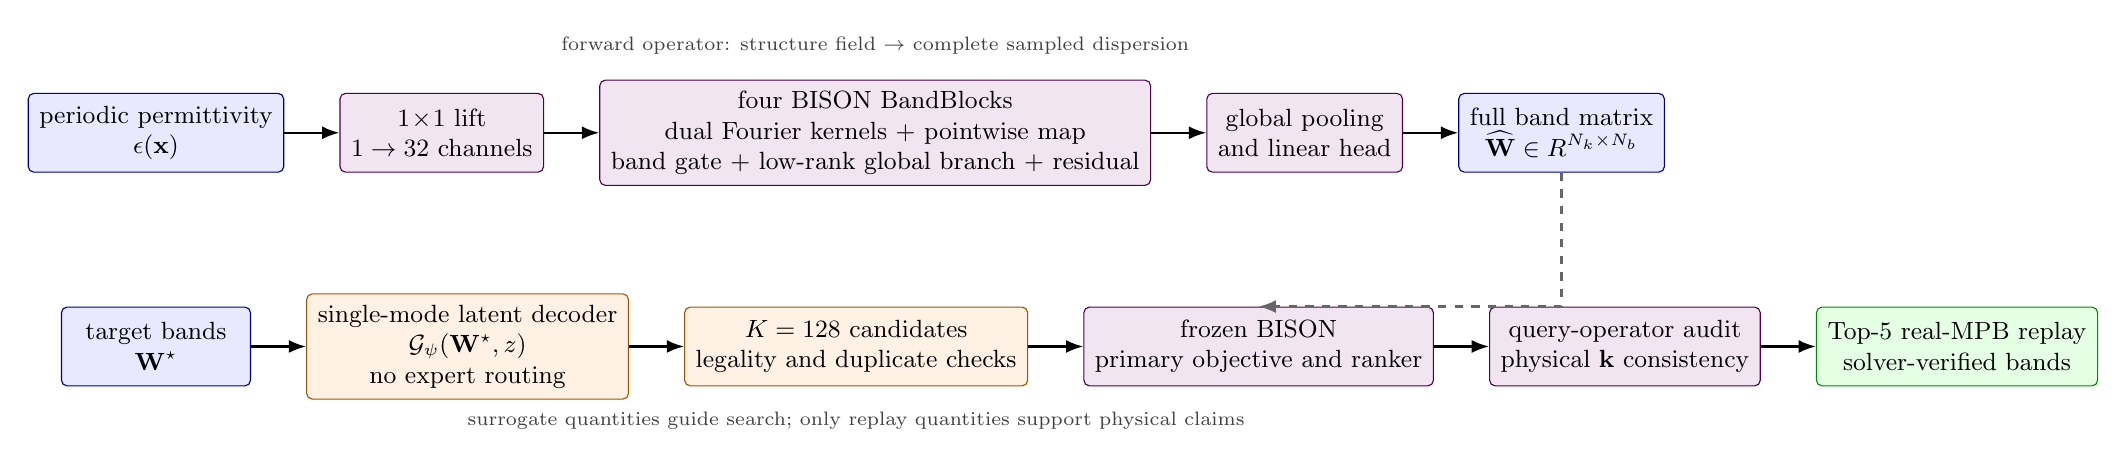
\begin{tikzpicture}[
    node distance=5mm and 7mm,
    box/.style={draw, rounded corners=2pt, align=center, minimum height=10mm,
      minimum width=24mm, inner sep=4pt, font=\small},
    data/.style={box, fill=blue!9, draw=blue!55!black},
    operator/.style={box, fill=violet!10, draw=violet!60!black},
    inverse/.style={box, fill=orange!11, draw=orange!65!black},
    solver/.style={box, fill=green!10, draw=green!55!black},
    note/.style={align=center, font=\scriptsize, text=black!75},
    arrow/.style={-{Latex[length=2.2mm]}, thick},
    audit/.style={-{Latex[length=2.2mm]}, thick, dashed, draw=black!60}
  ]
    \node[data] (eps) {periodic permittivity\\\(\permittivity(\mathbf{x})\)};
    \node[operator, right=of eps] (lift) {\(1\!\times\!1\) lift\\\(1\rightarrow32\) channels};
    \node[operator, right=of lift, minimum width=43mm] (blocks) {four BISON BandBlocks\\dual Fourier kernels $+$ pointwise map\\band gate $+$ low-rank global branch $+$ residual};
    \node[operator, right=of blocks] (pool) {global pooling\\and linear head};
    \node[data, right=of pool] (bands) {full band matrix\\\(\bandpred\in\mathbb{R}^{N_k\times N_b}\)};

    \draw[arrow] (eps) -- (lift);
    \draw[arrow] (lift) -- (blocks);
    \draw[arrow] (blocks) -- (pool);
    \draw[arrow] (pool) -- (bands);
    \node[note, above=2mm of blocks] {forward operator: structure field $\rightarrow$ complete sampled dispersion};

    \node[data, below=17mm of eps] (target) {target bands\\\(\bandtarget\)};
    \node[inverse, right=of target] (gen) {single-mode latent decoder\\\(\generator(\bandtarget,z)\)\\no expert routing};
    \node[inverse, right=of gen] (cand) {\(K=128\) candidates\\legality and duplicate checks};
    \node[operator, right=of cand] (rank) {frozen BISON\\primary objective and ranker};
    \node[operator, right=of rank] (query) {query-operator audit\\physical \(\mathbf{k}\) consistency};
    \node[solver, right=of query] (replay) {Top-5 real-MPB replay\\solver-verified bands};

    \draw[arrow] (target) -- (gen);
    \draw[arrow] (gen) -- (cand);
    \draw[arrow] (cand) -- (rank);
    \draw[arrow] (rank) -- (query);
    \draw[arrow] (query) -- (replay);
    \draw[audit] (bands.south) |- (rank.north);
    \node[note, below=2mm of cand] {surrogate quantities guide search; only replay quantities support physical claims};
  \end{tikzpicture}}
  \caption{BISON and the evidence-separated inverse-design loop. The upper row
  is the implemented full-band FNO-derived surrogate (registered in the code as
  \texttt{fno2d\_band\_v2}). The lower row uses the frozen operator to guide a
  no-expert latent candidate generator. The independent query model is an audit
  rather than a second equal-weight ranker, and MPB remains outside training.}
  \Description{Two-row workflow diagram. The upper row maps a periodic
  permittivity field through a lift, four BISON spectral blocks, pooling, and a
  linear head to a full band matrix. The lower row maps target bands through a
  single-mode latent generator, candidate checks, frozen BISON ranking, a query
  audit, and Top-5 MPB replay.}
  \label{fig:architecture}
\end{figure*}


% Related work for the BISON manuscript.
% Author: fangtoast
% Email: fangtoast@foxmail.com
% Copyright (c) 2026 fangtoast. All rights reserved.

\section{Related Work}

\subsection{From Solver-Based Photonic Design to Learned Search}

MPB solves the frequency-domain Maxwell eigenproblem in a plane-wave basis
~\cite{johnson2001mpb}. Topology optimization couples such physical models to
gradient-based search over many material degrees of freedom
~\cite{molesky2018inverse}. This approach has produced low-loss photonic-crystal
bends~\cite{jensen2004systematic}, nanophotonic components, and
dispersion-shaped or manufacturing-robust waveguides
~\cite{jensen2011topology,wang2011robust}. Grating couplers, wavelength
demultiplexers, and fabrication-constrained devices further demonstrate the
scope of solver-coupled optimization
~\cite{piggott2014grating,piggott2015demultiplexer,piggott2017fabrication}.
Its main computational cost is the repeated solution of a new physical problem
for each objective and design iterate.

Learned surrogates shift part of this cost to dataset generation and training.
They have accelerated nanoparticle simulation, power-splitter design, and
global design-space exploration
~\cite{peurifoy2018nanophotonic,tahersima2019splitters,melati2019mapping}.
Tandem networks address inverse non-uniqueness by training through a frozen
forward surrogate~\cite{liu2018tandem}, whereas conditional generators and
global-optimization networks search over multiple candidates
~\cite{jiang2019glonet}. Across direct, iterative, and generative approaches,
the recurring concerns are non-uniqueness, data coverage, surrogate bias, and
physical validation~\cite{so2020inverse,ma2021deep,wiecha2021deep,
jiang2021evaluation}. Budget-aware evaluation is therefore essential
~\cite{ren2020benchmarking}. Our protocol fixes both the \(K=128\) candidate
pool and the Top-5 MPB replay budget.

\subsection{Neural Operators and Fourier-Space Inductive Bias}

DeepONet represents nonlinear operators with branch and trunk networks
~\cite{lu2021deeponet}. FNO alternates pointwise transformations with global
convolutions parameterized by learned Fourier modes~\cite{li2021fno}. Both fit
within the broader framework of learning maps between function spaces
~\cite{kovachki2023neuraloperator}. Subsequent variants extend Fourier mixing
or geometry handling. AFNO adds adaptive sparsification and channel structure
~\cite{guibas2022afno}, Geo-FNO deforms irregular domains to a uniform latent
grid~\cite{li2023geofno}, and NUNO decomposes non-uniform domains into
grid-aligned subdomains~\cite{liu2023nuno}.

BISON addresses a narrower setting with a stronger structural prior: a fixed
periodic Cartesian cell. It specializes Fourier mixing to two configured mode
rectangles and jointly predicts an ordered band matrix. Unlike
physics-informed neural operators, which can incorporate equation residuals
~\cite{li2021pino}, BISON is trained on paired permittivity and eigenspectrum
data. Neural Inverse Operators instead learn operator compositions for PDE
inverse problems~\cite{molinaro2023nio}. In this paper, ``operator'' denotes the
learned functional map from a permittivity field to a finite sampled
eigenspectrum.

\subsection{Learned Electromagnetics and Photonic Band Surrogates}

Learned electromagnetic models differ in both prediction target and validation
evidence. MaxwellNet incorporates Maxwell-equation residuals into field
prediction~\cite{lim2022maxwellnet}. NeurOLight and PACE use neural operators
for parametric photonic-device field simulation
~\cite{gu2022neurolight,zhu2024pace}, and an operator surrogate has supported
free-form electromagnetic inverse design~\cite{augenstein2023emno}. Field
solutions, port responses, and ordered eigenfrequency matrices nevertheless
define different learning tasks and require different evaluation protocols.

Christensen et al. predict complete band structures and generate band-gap
candidates for two-dimensional photonic crystals
~\cite{christensen2020predictive}. POD--DeepONet similarly studies forward and
inverse band design on binary, symmetric two-dimensional cells
~\cite{wang2026poddeeponet}. Direct accuracy comparisons are not warranted
because the datasets, discretizations, targets, and replay protocols differ.
BISON instead combines joint full-band prediction with a routing-free latent
generator, an independent query audit, and equal candidate and MPB budgets.

\begin{table*}[t]
  \caption{Positioning of BISON among photonic inverse-design methods.
  ``Physical check'' summarizes the typical evidence type; solvers and budgets
  differ across the cited studies.}
  \label{tab:positioning}
  \centering
  \small
  \begin{tabular}{@{}p{0.18\textwidth}p{0.20\textwidth}p{0.20\textwidth}p{0.17\textwidth}p{0.17\textwidth}@{}}
    \toprule
    Family & Learned or optimized object & Main advantage & Main risk or cost & Physical check \\
    \midrule
    Topology/adjoint design & One structure per objective & Direct solver gradients & Many iterative solves & In-loop or final solver \\
    Direct/tandem learning & Target response $\rightarrow$ structure & Fast amortized inference & One-to-many ambiguity; surrogate bias & Often post-hoc simulation \\
    Generative/search learning & Candidate distribution or latent search & Multiple feasible designs & Budget-sensitive ranking & Candidate-dependent \\
    Photonic neural operators & Geometry/conditions $\rightarrow$ fields or response & Global functional mapping & Distribution shift & Field/response solver \\
    BISON workflow & Periodic cell $\rightarrow$ full bands; latent candidates & Joint band ranking with explicit budgets & Fixed task family; surrogate error & Top-5 MPB replay per target \\
    \bottomrule
  \end{tabular}
\end{table*}

% Problem formulation for the BISON manuscript.
% Author: fangtoast
% Email: fangtoast@foxmail.com
% Copyright (c) 2026 fangtoast. All rights reserved.

\section{Problem Formulation}

Let \(\design\in\{0,1\}^{H\times W}\) denote a binary material layout on a
square periodic unit cell. The dataset enforces \(\pgroup\) symmetry, and the
permittivity is
\begin{equation}
  \permittivity(\mathbf{x})=\epsilon_{\mathrm{air}}+
  (\epsilon_{\mathrm{mat}}-\epsilon_{\mathrm{air}})\design(\mathbf{x}).
  \label{eq:permittivity}
\end{equation}
For sampled Bloch vectors
\(\kpath=\{\mathbf{k}_i\}_{i=1}^{N_k}\), an MPB eigensolve defines the
forward map
\begin{equation}
  \mathcal{F}^{\star}:\permittivity\longmapsto
  \mathbf{W}=[\omega_{i,b}]\in\mathbb{R}^{N_k\times N_b},
  \label{eq:physical-forward}
\end{equation}
where frequencies are normalized by \(a/(2\pi c)\). BISON learns
\(\bandop\approx\mathcal{F}^{\star}\) from paired structures and band
matrices. The implementation reads \(H,W,N_k,N_b\) from the data schema; the
reported dataset instance has \(H=W=16\), \(N_k=31\), and \(N_b=10\).

Predicting \(\mathbf{W}\) jointly matters for inverse design. A target can
specify a local gap, a band slope, or a multi-band profile, but each objective
is evaluated within one ordered eigenspectrum. Independent scalar regressors
would discard correlations across neighboring wave vectors and bands. BISON
therefore produces the full \(N_k\times N_b\) matrix in one pass, even though
the frozen inverse metric later excludes band 1 for numerical reasons.

Given a target \(\bandtarget\), inverse design seeks one or more legal
structures whose solver response matches that target. A latent conditional
generator produces
\begin{equation}
  \widehat{\design}_{j}=\generator(\bandtarget,\mathbf{z}_j),
  \qquad \mathbf{z}_j\sim\mathcal{N}(\mathbf{0},\mathbf{I}),
  \quad j=1,\ldots,K.
  \label{eq:inverse-generation}
\end{equation}
Because multiple structures can realize similar spectra, recovery of the
paired training geometry is not the objective. We instead evaluate spectral
realization. For bands \(\mathcal{B}=\{2,\ldots,N_b\}\), the per-target mean
relative error is
\begin{equation}
  \mre(\mathbf{A},\mathbf{B})=
  \frac{100}{N_k|\mathcal{B}|}
  \sum_{i=1}^{N_k}\sum_{b\in\mathcal{B}}
  \frac{|A_{i,b}-B_{i,b}|}{|B_{i,b}|}.
  \label{eq:mre}
\end{equation}
Band 1 is excluded by the frozen protocol because its near-zero values make a
relative metric ill-conditioned.

The inverse problem is thus not posed as estimating a unique
\(\mathcal{F}^{\star-1}\). It is a constrained selection problem: sample a set
of legal geometries, rank them cheaply with learned operators, and spend a
limited solver budget on the most promising distinct candidates. This
formulation makes the candidate count \(K\), deduplication rule, and replay
count part of the experimental definition rather than hidden implementation
details.

The evaluation has three distinct evidence levels. A
\emph{surrogate-only} value compares \(\bandop(\widehat{\design})\) with the
target. A \emph{cross-surrogate audit} additionally compares a second model
queried at physical \(\mathbf{k}\) coordinates. A \emph{solver-verified}
value evaluates \(\mpb(\widehat{\design})\). The first two guide search and
diagnose distribution shift; only the third supports a physical claim.

% Method section for the BISON manuscript.
% Author: fangtoast
% Email: fangtoast@foxmail.com
% Copyright (c) 2026 fangtoast. All rights reserved.

\section{Method}

\subsection{Band-Informed Spectral Operator}

BISON consumes \(\permittivity\) as a one-channel periodic field. A
\(1\times1\) convolution first lifts it to \(C\) latent channels,
\(\mathbf{u}_0=P\permittivity\). Four BandBlocks then update the field. In
block \(\ell\), the spectral path is
\begin{equation}
  \mathbf{s}_{\ell}=\mathcal{F}^{-1}\!\left[
  \left(R^{\mathrm{full}}_{\ell}+R^{\mathrm{band}}_{\ell}\right)
  \mathcal{F}(\mathbf{u}_{\ell})\right],
  \label{eq:dual-spectral}
\end{equation}
where both complex kernels act on configured low-frequency rectangles, with
the band kernel using a separately configured subset. The two kernels are
learned independently and added in Fourier space. A pointwise convolution is
combined with this global path, then modulated by a learned sigmoid gate:
\begin{align}
  \mathbf{a}_{\ell}&=\mathbf{s}_{\ell}+W_{\ell}\mathbf{u}_{\ell},\\
  \widetilde{\mathbf{a}}_{\ell}
  &=\sigma(G_{\ell}\mathbf{a}_{\ell})\odot\mathbf{a}_{\ell}.
\end{align}
A low-rank global branch pools the residual field, applies
\(C\rightarrow r\rightarrow C\) channel maps, and broadcasts the result.
The block output is
\begin{equation}
  \mathbf{u}_{\ell+1}=\operatorname{GELU}\!\left(
  S_{\ell}[\widetilde{\mathbf{a}}_{\ell}+L_{\ell}(\mathbf{u}_{\ell})]
  +\mathbf{u}_{\ell}\right).
  \label{eq:bandblock}
\end{equation}
Adaptive global pooling followed by a linear head reshapes the final channels
to \(\bandpred\in\mathbb{R}^{N_k\times N_b}\). In the evaluated configuration,
\(C=32\), \(r=8\), the two spectral rectangles retain \(8\times8\) and
\(5\times5\) modes, four BandBlocks are stacked, and the network contains
389,718 trainable parameters. Both Fourier weights are complex-valued and are
cropped at runtime when the data grid provides fewer available modes.

Figure~\ref{fig:bison-detailed} expands this implemented operator at both the
network and block levels. It makes explicit that the band gate acts on the
sum of the global spectral and local pointwise paths, while the pooled
low-rank branch is computed from the block input and broadcast before the
learned projection and identity residual.

\begin{figure*}[t]
  \centering
  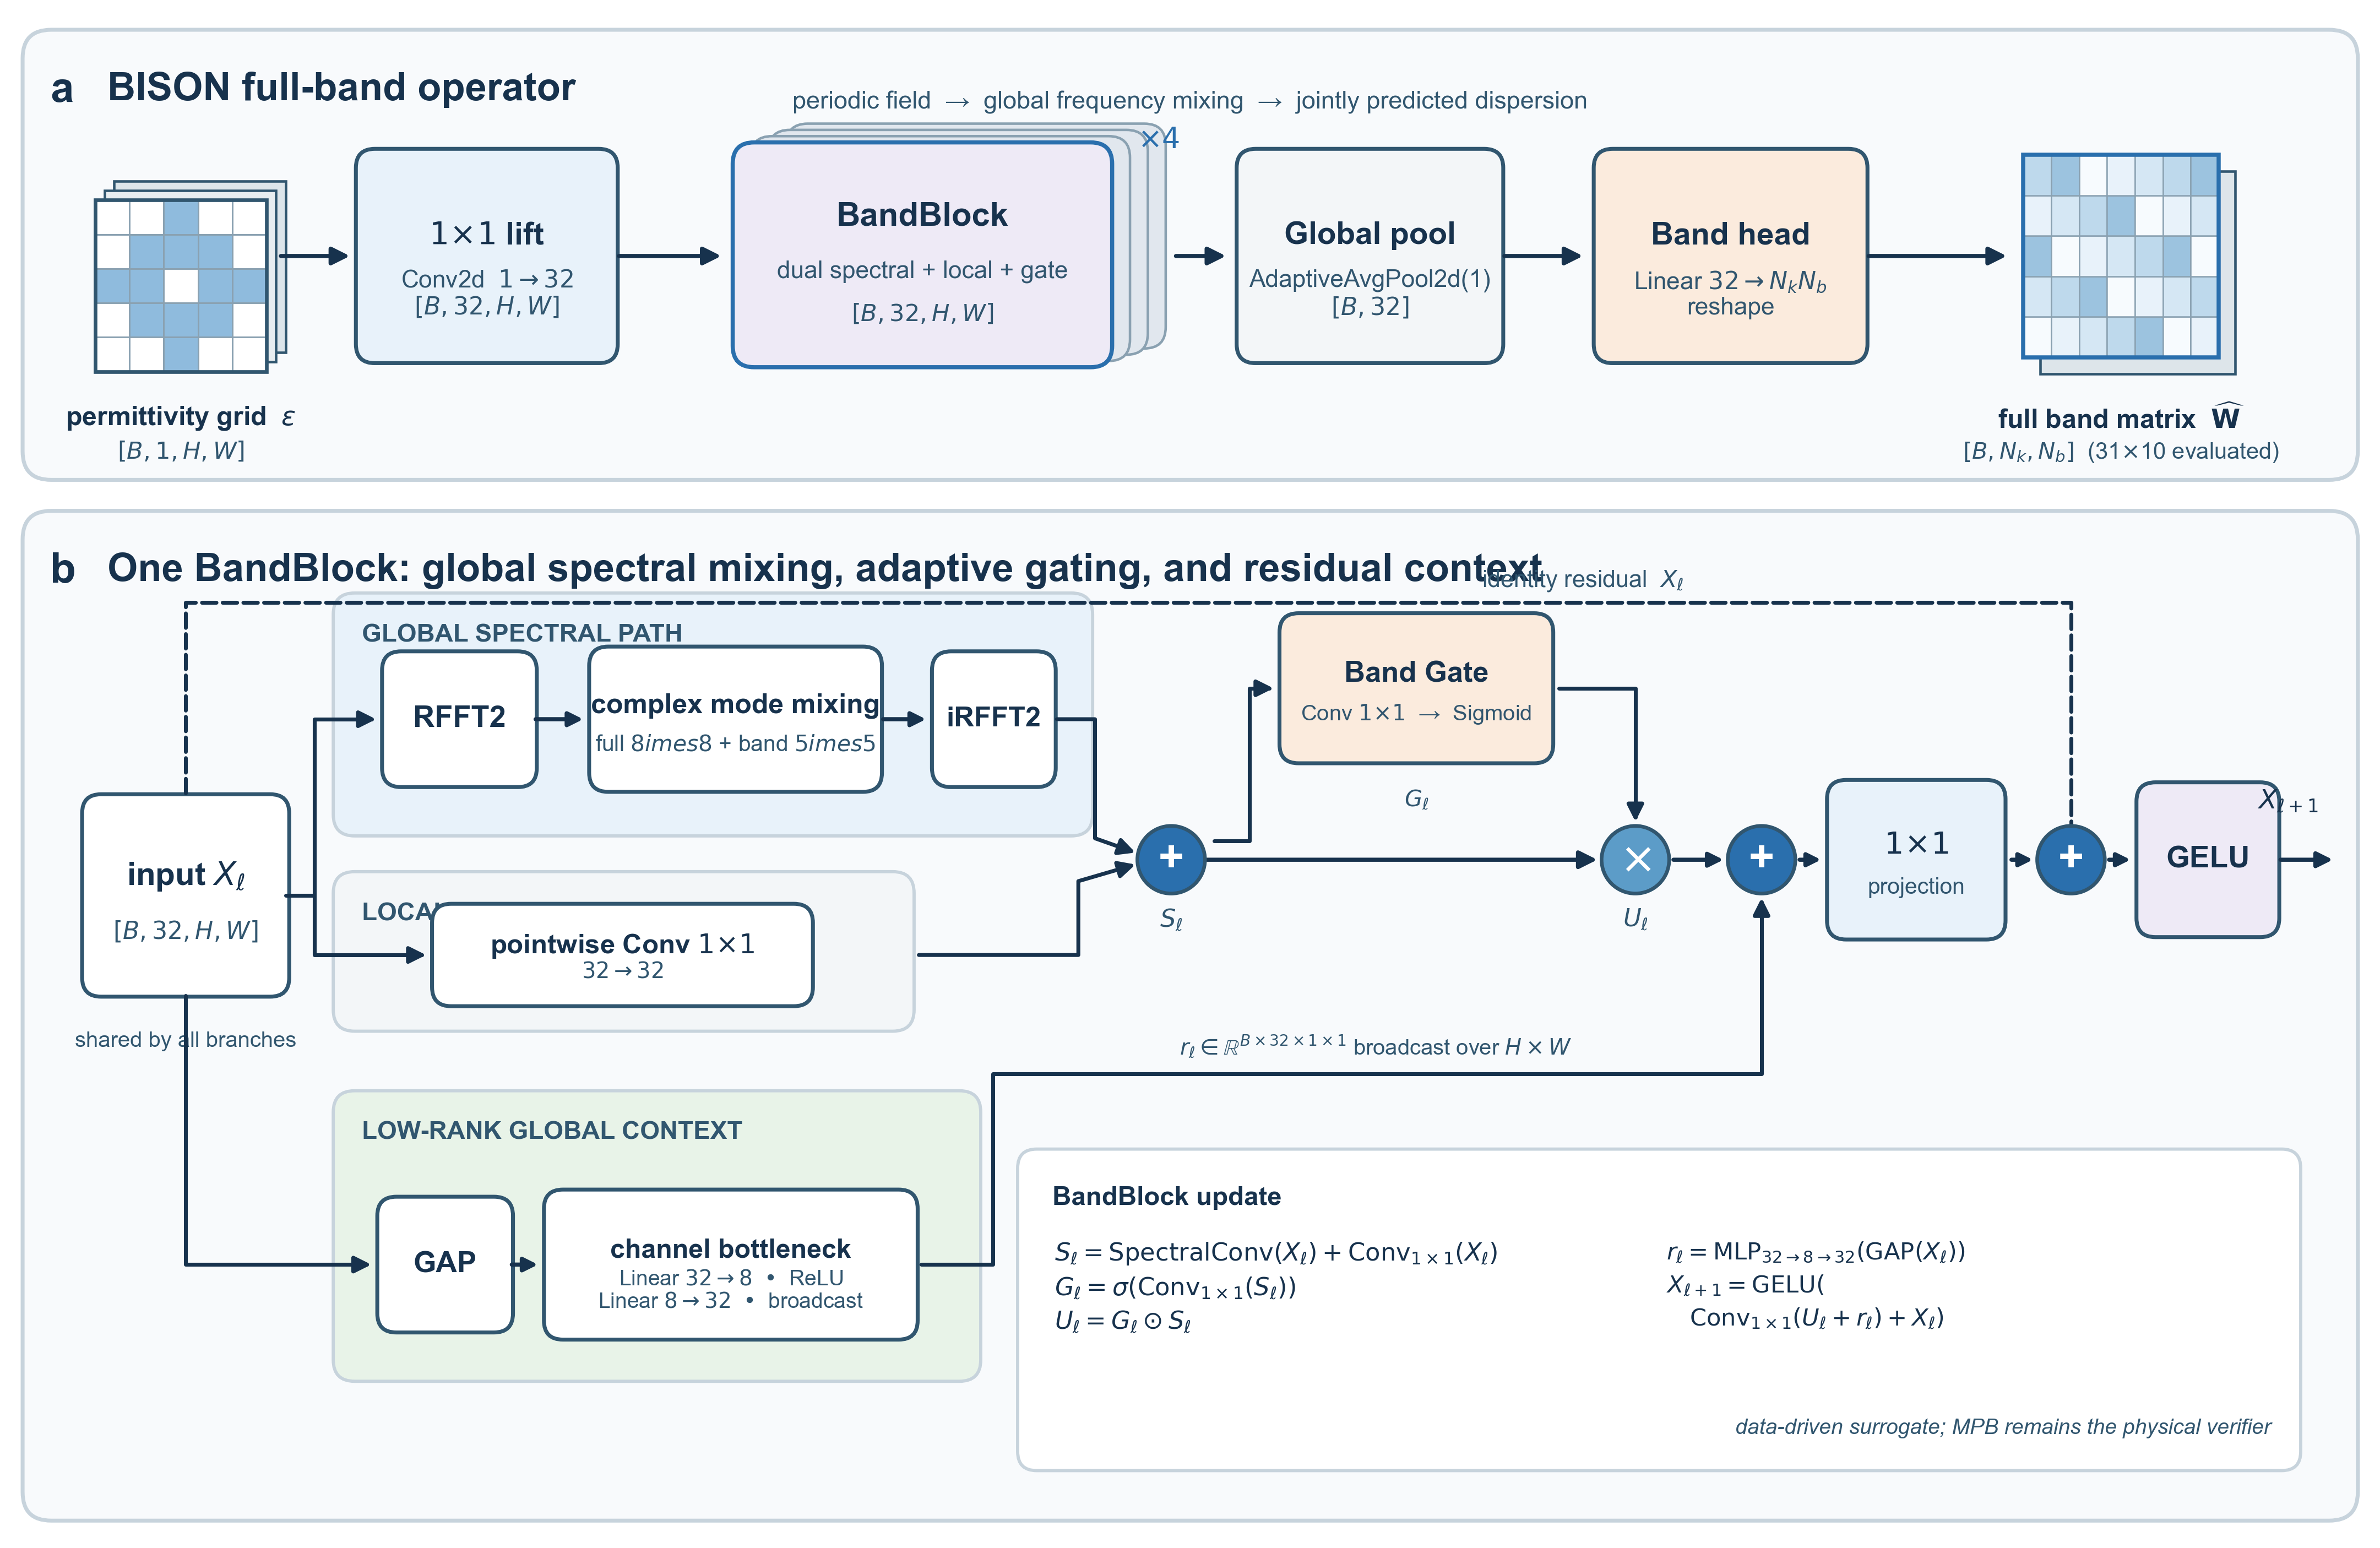
\includegraphics[width=\textwidth]{figures/bison_architecture_detailed.png}
  \caption{Detailed architecture of the BISON forward operator.
  \textbf{(a)} A periodic permittivity grid is lifted to \(C=32\) channels,
  processed by four BandBlocks, globally pooled, and mapped jointly to the
  ordered \(N_k\times N_b\) band matrix (\(31\times10\) in the evaluated A1
  data). \textbf{(b)} Inside one BandBlock, an RFFT2 branch mixes two learned
  complex low-mode rectangles (configured as \(8\times8\) and \(5\times5\))
  and is added to a local \(1\times1\) path. A sigmoid channel gate modulates
  this mixed field. In parallel, global average pooling and the
  \(32\rightarrow8\rightarrow32\) bottleneck produce a broadcast context
  vector. Their sum passes through a learned \(1\times1\) projection before
  the identity residual and GELU activation. The diagram follows the actual
  implementation order; it depicts a data-driven surrogate rather than an
  embedded MPB or Maxwell solver.}
  \Description{A two-panel architecture diagram. Panel a shows a permittivity
  grid flowing through a one-by-one lift, four stacked BandBlocks, global
  pooling, and a linear band head to a full band matrix. Panel b expands a
  BandBlock into spectral, pointwise, gating, low-rank global-context,
  projection, residual, and activation paths.}
  \label{fig:bison-detailed}
\end{figure*}

The architecture is FNO-derived rather than a separate physics solver. Its
inductive bias is that periodic geometry and long-range interactions are
processed globally in Fourier space, while the full ordered band matrix is
predicted jointly. This paper uses the name BISON for this exact implemented
model, not for a hypothetical replacement architecture.

The term \emph{band-informed} refers to this task specialization, not to a
hard-coded Maxwell constraint. The second spectral kernel gives the block a
separate learnable low-mode scale; the sigmoid gate determines which mixed
channels are passed onward; and the pooled bottleneck injects a cell-wide
summary before the residual update. Their combined output is learned solely
from paired permittivity--band data. Consequently, the architecture can be a
fast spectral surrogate, but its predictions still require calibration and
solver replay when used outside ordinary held-out forward evaluation.

\subsection{Independent Query-Operator Audit}

The project also trains \(\queryop(\permittivity,\mathbf{k})\), which returns
the band vector at a physical Bloch coordinate. It is evaluated on all sampled
queries, interpolation points withheld from otherwise observed path segments,
and a completely held-out path segment. During inverse evaluation, BISON is
the primary objective and ranker; \(\queryop\) is a diagnostic consistency
gate. This asymmetric use avoids presenting agreement between two learned
models as physical verification.

\subsection{Single-Mode No-Expert Candidate Generator}

For inverse design, the target matrix is flattened and encoded by two
GELU-activated linear layers. The encoded condition is concatenated with a
32-dimensional Gaussian latent vector and one fixed mode embedding, then
decoded by a four-layer, width-256 MLP with a sigmoid output. Setting the mode
count to one removes routing and expert selection: every draw is processed by
the same parameters and differs only through its continuous latent vector.
The output represents the independent degrees of freedom of the symmetric
binary design; deterministic lifting and thresholding recover the complete
\(\pgroup\) unit cell.

The inverse model is warm-started from paired reconstruction and then optimized
for 50 epochs with AdamW while BISON and the query operator remain frozen. For
16 latent candidates per training condition, the objective is
\begin{equation}
\begin{split}
  \mathcal{L}={}&\mathcal{L}_{\mathrm{BISON}}
  +0.03\mathcal{L}_{\mathrm{rec}}
  +0.20\mathcal{L}_{\mathrm{div}}
  +0.50\mathcal{L}_{\mathrm{bin\text{-}div}}\\
  &+0.25\mathcal{L}_{\mathrm{latent}}
  +0.90\mathcal{L}_{\mathrm{collision}}
  +0.20\mathcal{L}_{\mathrm{cross}}
  +0.20\mathcal{L}_{\mathrm{gap}}.
  \label{eq:inverse-objective}
\end{split}
\end{equation}
The terms promote target fidelity, paired warm-start stability, continuous and
binary diversity, latent responsiveness, separation from near-duplicate
structures, and agreement between the two frozen surrogates. MPB gradients are
not used.

This generator is intentionally subordinate to BISON in the paper's method
identity. BISON defines the learned full-band objective; the generator proposes
points in the legal design space. Calling the combined system a mixture of
experts would be misleading because the selected method has one fixed mode,
one decoder, and no learned router. The four-mode version is retained only as a
same-implementation baseline for testing whether discrete mode embeddings add
value under an identical sampling budget.

\subsection{Candidate Ranking and Solver Replay}

At inference, each target receives \(K=128\) latent draws. Candidates are
thresholded at 0.5, checked for legality, and deduplicated using a normalized
Hamming threshold determined by the geometry degrees of freedom. Frozen BISON
ranks the surviving pool by bands-2--10 MRE; the query model records an
independent diagnostic score. The five best BISON-ranked candidates are then
recomputed by MPB, and the lowest real-MPB MRE is reported. The mode-count-four
generator is evaluated only as a same-budget baseline. It is not part of
BISON and is not required by the proposed no-expert workflow.

% Experimental protocol for the BISON manuscript.
% Author: fangtoast
% Email: fangtoast@foxmail.com
% Copyright (c) 2026 fangtoast. All rights reserved.

\section{Experimental Protocol}

The evaluation follows the same evidence chain throughout.
\textbf{RQ1} tests full-band prediction against dense and local-convolution
baselines on unseen structures. \textbf{RQ2} evaluates a
coordinate-conditioned operator at withheld interpolation points and on an
unseen path segment. \textbf{RQ3} tests whether candidates ranked by BISON
retain their paired advantage after equal-budget MPB replay. Forward accuracy
alone is not used to infer inverse-design performance.

\subsection{Dataset and Physical Solver}

The MPB-generated dataset contains 10,000 binary,
\(\pgroup\)-symmetric unit cells on a \(16\times16\) grid. Each sample
contains 10 transverse-electric bands at 31 ordered wave-vector points. The
fixed split comprises 6,875 training, 2,500 validation, and 625 test
structures. All forward, query, and inverse evaluations reuse these structure
identities. The solver uses \(\epsilon_{\mathrm{air}}=1.0\),
\(\epsilon_{\mathrm{mat}}=8.9\), lattice constant \(a=1\), resolution 64,
10 bands, and eigensolver tolerance \(10^{-7}\).

The split unit is a complete structure and its band matrix. Wave-vector rows
from one structure are not divided between training and test sets. Query
partitions are constructed within the same structure identities. Interpolation
and held-segment tests therefore probe wave-vector generalization without
altering the structural test set.

\subsection{Forward and Query Comparisons}

The formal forward comparison includes BISON, a wide residual MLP, a lifted
CNN, and a plain MLP. Each model predicts the complete \(31\times10\) band
matrix from the input representation specified by the fair-comparison
protocol. Learning rates are selected on the validation split. Bands-2--10
test MRE is reported as the mean and standard deviation over seeds 0, 1, and
2. Each run also records parameter count, training time, inference latency,
and peak memory.

For the query task, each input pairs a structure with a physical wave vector,
and the output is a 10-band vector. We compare the FNO query model, DeepONet,
and an MLP under three protocols: the full path for unseen structures
(all-\(k\)), withheld interpolation points, and a contiguous held-out path
segment. The latter two protocols separate interpolation from path
extrapolation.

All model selection uses validation data, and the test set is reserved for the
reported estimates. The same bands-2--10 MRE definition is used for each
full-band comparison. Query evaluation reports band-order violations
separately because pointwise error and spectral ordering measure different
properties.

\subsection{Inverse Replay Protocol}

The inverse evaluation reuses frozen seed-0 BISON and query checkpoints; no
test target participates in checkpoint selection. All 625 test band matrices
receive a fixed pool of 128 candidates and a Top-5 MPB replay budget. The
single-mode routing-free generator is compared with the same decoder configured
with four cyclic mode embeddings. Both variants use latent width 32, hidden
width 256, depth four, identical objective weights, checkpoint-selection
rules, and replay budgets. Earlier retrieval and direct-inverse results are
excluded because the complete-test extension did not replay them.

This controlled comparison tests whether multiple fixed mode embeddings
improve the implemented latent decoder. It does not compare broader
generative-model families. The single-mode variant samples a continuous latent
distribution, and BISON provides the candidate ranking.

MPB replay uses eight isolated worker processes, failure-on-error semantics,
frequency-ascending band order, and structure-hash caching. Evaluation reports
the best of five replayed candidates per target. Confidence intervals use
10,000 bootstrap resamples, and the paired comparison includes a two-sided
sign test.

\subsection{Metrics and Reproducibility Boundary}

Forward results use the percentage MRE in Eq.~\eqref{eq:mre}. Inverse metrics
include surrogate MRE, real-MPB MRE, their difference in percentage points,
median replay MRE, and the effective unique candidate count. Runtime is
separated into candidate sampling, surrogate ranking, and solver replay.
Formal runs were executed in WSL Ubuntu with the
\texttt{meep\_env} Conda environment, PyTorch/CUDA in FP32 on an NVIDIA RTX
4060 Laptop GPU; MPB was invoked through the same environment. Appendix
\ref{app:provenance} records the artifact hashes and exact claim boundary.

% Results for the BISON manuscript.
% Author: fangtoast
% Email: fangtoast@foxmail.com
% Copyright (c) 2026 fangtoast. All rights reserved.

\section{Results}

We present results in the same order as the evidence chain: forward surrogate
quality (RQ1), query-space robustness (RQ2), and solver-verified inverse design
(RQ3). Each subsection closes with what the measurement establishes and what
it leaves unresolved.

\subsection{BISON Improves Full-Band Prediction}

Table~\ref{tab:forward} shows the formal three-seed comparison. BISON obtains
\(1.0299\%\pm0.0545\%\) test MRE, compared
with \(1.3309\%\pm0.0122\%\) for the strongest non-operator baseline,
ResMLP-wide. This is a 22.6\% relative reduction. The lifted CNN and plain MLP
are less accurate at 2.2234\% and 2.4764\%, respectively. The improvement is
not explained by parameter count alone: BISON uses 389,718 parameters, less
than half the 878,646 parameters of either MLP model.

\begin{table}[t]
  \caption{Formal forward comparison on the 625-structure test split. MRE and
  training time are mean\(\pm\)standard deviation over three seeds; latency and
  peak memory are means across seeds.}
  \label{tab:forward}
  \centering
  \small
  \resizebox{\columnwidth}{!}{%
  \begin{tabular}{lrrrr}
    \toprule
    Model & MRE (\%) $\downarrow$ & Params & Train (s) & ms/sample \\
    \midrule
    \method{} & $\mathbf{1.0299\pm0.0545}$ & 389,718 & 272.71 & 0.5267 \\
    ResMLP-wide & $1.3309\pm0.0122$ & 878,646 & 80.96 & 0.0064 \\
    Lifted CNN & $2.2234\pm0.0366$ & 5,458 & 39.97 & 0.0102 \\
    MLP & $2.4764\pm0.0241$ & 878,646 & 65.66 & 0.0074 \\
    \bottomrule
  \end{tabular}}
\end{table}

BISON's best per-band result is band 4 (0.9028\% MRE), while band 10 is the
hardest (1.2765\%). Thus, the gain is distributed across the band matrix rather
than arising from a single easy output. The cost is higher training and
inference time than the small dense baselines, although sub-millisecond
inference remains negligible relative to eigensolver replay.

RQ1 is therefore answered within the fixed dataset and metric: the implemented
spectral operator gives the lowest three-seed held-out full-band MRE among the
four tested models. This comparison does not isolate which BandBlock component
causes the gain, nor does it establish resolution or lattice transfer.

\subsection{Query Interpolation Works Better than Extrapolation}

The FNO query model records \(1.1004\%\pm0.0218\%\) MRE on unseen structures
over all sampled wave vectors and \(1.0470\%\pm0.0240\%\) on withheld
interpolation queries. On a held-out path segment, its error rises to
\(3.6747\%\pm0.1730\%\) and its band-order violation rate rises from 2.16\%
under interpolation to 9.22\%. This is an important negative result: physical
coordinates allow flexible queries, but they do not by themselves guarantee
reliable extrapolation.

\begin{table}[t]
  \caption{Three-seed query prediction. Values are MRE (\%) and band-order
  violation rate (\%).}
  \label{tab:query}
  \centering
  \small
  \resizebox{\columnwidth}{!}{%
  \begin{tabular}{lrrrrrr}
    \toprule
     & \multicolumn{2}{c}{All-$k$} & \multicolumn{2}{c}{Interpolation}
     & \multicolumn{2}{c}{Held segment} \\
    Model & MRE & Viol. & MRE & Viol. & MRE & Viol. \\
    \midrule
    FNO query & \textbf{1.1004} & 2.96 & \textbf{1.0470} & 2.16 & \textbf{3.6747} & 9.22 \\
    DeepONet & 1.7937 & 1.35 & 1.6308 & \textbf{0.41} & 3.7604 & \textbf{0.99} \\
    MLP query & 2.1800 & \textbf{0.83} & 2.2079 & 0.42 & 4.2548 & 1.00 \\
    \bottomrule
  \end{tabular}}
\end{table}

DeepONet has lower ordering-violation rates despite higher MRE, showing that
point accuracy and physical ordering are distinct. For this reason the query
network is retained as an audit signal, not treated as an unquestionable
second oracle.

RQ2 has a mixed answer. The coordinate-conditioned FNO interpolates held-out
points accurately, but neither the coordinate input nor the operator backbone
prevents a large error increase on an unseen path segment. The negative result
supports using the query model as a distribution-shift diagnostic rather than
as a substitute for MPB.

\subsection{No-Expert Inverse Design Survives MPB Replay}

On all 625 test targets, the one-mode generator reaches 2.1434\% BISON MRE and
2.2614\% real-MPB MRE (Table~\ref{tab:inverse}). The resulting
surrogate--replay gap is 0.118 percentage points. Its replay distribution has
median 2.2196\%, 10th percentile 1.7264\%, and 90th percentile 2.8262\%; the
95\% bootstrap interval for its mean is [2.2263, 2.2965]\%.

\begin{table}[t]
  \caption{Seed-0 inverse evaluation on the complete 625-target test split.
  Both methods use $K=128$ and Top-5 MPB replay. CI is the 95\% bootstrap
  interval of mean MPB MRE. Gap is MPB minus BISON MRE in percentage points.}
  \label{tab:inverse}
  \centering
  \small
  \resizebox{\columnwidth}{!}{%
  \begin{tabular}{lrrrrr}
    \toprule
    Generator & BISON & MPB (\%) & 95\% CI & Gap (pp) & Eff. $K$ \\
    \midrule
    Single mode (ours) & \textbf{2.1434} & \textbf{2.2614} & [2.2263,2.2965] & \textbf{0.1180} & \textbf{112.02} \\
    Four modes & 2.2477 & 2.3916 & [2.3485,2.4341] & 0.1440 & 109.24 \\
    \bottomrule
  \end{tabular}}
\end{table}

Under the identical candidate and solver budget, the four-mode baseline has
2.3916\% MPB MRE. The paired difference (four-mode minus one-mode) is 0.1302
percentage points, with bootstrap interval [0.0905, 0.1705] and two-sided sign
test \(p=0.0010\). The result supports the narrower conclusion that expert-like
mode routing was unnecessary in this seed-0 protocol. It does not establish a
universal architectural advantage or cross-seed stability.

RQ3 is answered only at the strength of this protocol: for the complete
625-target split and one training seed, BISON-ranked single-mode candidates
retain a statistically consistent paired advantage after the same five MPB
replays per target. The solver gap is nonzero, so the result validates the
budgeted workflow rather than certifying BISON as an exact physical model.
Figure~\ref{fig:inverse-examples} complements the aggregate result with four
paired examples selected jointly from the same complete replay.

\begin{figure*}[t]
  \centering
  % Canonical editable source: docs/.../inverse/paired_main4.svg
  \includegraphics[width=\textwidth]{../../docs/reports/assets/phc2d_project_full_introduction_20260724/inverse/paired_main4.pdf}
  \caption{Paired qualitative comparison between the single-mode no-expert
  generator and the four-mode mixture baseline in the seed-0, 625-target
  replay. Rows show the jointly selected best target, median target, largest
  between-method disagreement, and worst target. For each method, the figure
  displays the generated structure and the target, BISON-surrogate, and
  real-MPB band curves; the header reports MPB MRE, surrogate MRE, and their
  signed gap. These cases expose both ordinary paired behavior and difficult
  targets, but remain qualitative single-seed evidence.}
  \Description{Four rows compare single-mode and four-mode inverse-design
  candidates for jointly selected best, median, largest-disagreement, and
  worst targets. Each method column includes a generated binary unit cell,
  target and predicted band curves, MPB replay curves, and error summaries.}
  \label{fig:inverse-examples}
\end{figure*}

\subsection{Runtime and Evidence Boundary}

For the one-mode method, generating candidates for all 625 targets takes
1.408~s in total (2.25~ms/target), while BISON ranking takes 221.333~s
(354.13~ms/target). The effective pool contains 112.02 candidates on average
after binary deduplication. The query audit returns 2.1254\% MRE and differs
from BISON by 0.8457 percentage points under its own diagnostic definition;
this disagreement is retained rather than hidden.

The forward table is a formal three-seed result. The inverse table is a
complete-test but single-seed result. Earlier retrieval and direct-inverse
numbers, field/PINO residuals, and historical seed-2 comparisons are not used
as current inverse claims because they lack the same accepted replay protocol.

% Discussion, limitations, and ethics.
% Author: fangtoast
% Email: fangtoast@foxmail.com
% Copyright (c) 2026 fangtoast. All rights reserved.

\section{Discussion, Limitations, and Ethics}

The experiments suggest two complementary conclusions. First, Fourier-space
global coupling and joint full-band prediction provide a useful inductive bias:
BISON is more accurate than substantially larger dense models. Second, forward
accuracy is necessary but not sufficient for inverse design. The 0.118-point
surrogate--replay gap is small relative to the final error, yet individual
targets still fail more severely and the independent query model can disagree.
Retaining the MPB boundary is therefore part of the method, not an optional
post-processing detail.

The results also clarify why the method should be described as a system rather
than as a single forward benchmark. Full-band accuracy makes BISON useful for
ranking objectives that depend on several bands and wave vectors at once. The
query operator probes whether this score is consistent under a second output
factorization, while MPB decides whether the selected geometry actually
realizes the target. Removing either diagnostic would make the inverse claim
less interpretable: surrogate-only optimization hides exploitation, whereas
solver-only reporting hides how the replay budget was allocated.

Several limitations constrain the claim. The inverse experiment uses one
training seed, so its paired significance measures per-target consistency for
that frozen run rather than reproducibility across retraining. All structures
belong to one \(\pgroup\)-symmetric, binary, fixed-material design family on a
single path and resolution. We do not demonstrate transfer to arbitrary
lattices, multiple materials, three dimensions, alternative polarizations, or
fabrication-aware minimum features. The query result also shows poor held-path
extrapolation. Finally, no controlled ablation isolates every component of the
BandBlock; the present evidence supports the implemented BISON system as a
whole, not a causal claim for one gate or spectral branch.

These limitations define concrete next experiments. A component ablation
should remove the second spectral kernel, gate, and low-rank branch one at a
time under the same three-seed forward protocol. A multi-seed inverse study
should retrain both generator variants and repeat the complete 625-target
replay with identical candidate hashes and solver budgets. Resolution and
geometry transfer should compare schema-compatible grids without changing the
reported test identities, while fabrication-aware work should add minimum
feature and robustness constraints before any experimental realization claim.

The dataset is simulated and contains no personal or human-subject data. The
main broader risk is over-trusting a learned surrogate, which could waste
solver, fabrication, or laboratory resources. We mitigate this by publishing
surrogate and replay errors separately, reporting negative extrapolation and
worst-case examples, and requiring physical replay before describing a design
as realized.

% Generative AI disclosure.
% Author: fangtoast
% Email: fangtoast@foxmail.com
% Copyright (c) 2026 fangtoast. All rights reserved.

\section{Generative AI Usage}

A generative-AI coding and writing assistant was used to organize the
manuscript, improve English exposition, locate candidate literature, prepare
\LaTeX{} tables, and generate plotting code. Every numerical value in the
paper was recovered from local versioned run artifacts; citations were checked
against publisher, proceedings, or preprint records. The author remains
responsible for the scientific interpretation, evidence boundary, references,
figures, and final text.

% Conclusion for the BISON manuscript.
% Author: fangtoast
% Email: fangtoast@foxmail.com
% Copyright (c) 2026 fangtoast. All rights reserved.

\section{Conclusion}

We presented BISON, a project-specific, FNO-inspired spectral surrogate for
joint prediction of two-dimensional photonic-crystal band matrices. Across
three seeds, BISON achieved \(1.0299\%\pm0.0545\%\) forward MRE. In the
inverse workflow, a single-mode routing-free generator proposed 128 candidates
per target, BISON ranked them, and MPB replayed the Top-5 candidates. Evaluation
over all 625 test targets at seed 0 achieved 2.2614\% real-MPB MRE. This value
was 0.1302 percentage points below that of the four-mode embedding baseline
under the same budget. Query extrapolation error and the nonzero
surrogate--replay gap delimit the scope of the learned models. The results
support BISON as a ranking surrogate within this fixed dataset and replay
protocol, while MPB remains the final evaluator of the selected structures.


\bibliographystyle{ACM-Reference-Format}
\bibliography{references}

\appendix
% Reproducibility appendix for the BISON manuscript.
% Author: fangtoast
% Email: fangtoast@foxmail.com
% Copyright (c) 2026 fangtoast. All rights reserved.

\section{Reproducibility Details}

\subsection{BISON Configuration}

\begin{table}[H]
  \caption{Architecture and training configuration used for the formal forward
  BISON result. Output dimensions are supplied by the dataset schema.}
  \label{tab:bison-config}
  \centering
  \small
  \begin{tabular}{ll}
    \toprule
    Item & Value \\
    \midrule
    Input representation & periodic permittivity grid \\
    Lift width / BandBlocks & 32 / 4 \\
    Spectral modes / band modes & $8\times8$ / $5\times5$ \\
    Global low-rank width & 8 \\
    Activation & GELU \\
    Pooling / head & adaptive average / linear \\
    Output in this dataset & $31\times10$ bands \\
    Trainable parameters & 389,718 \\
    Selected learning rate & $10^{-3}$ \\
    Seeds & 0, 1, 2 \\
    Evaluation bands & 2--10 \\
    \bottomrule
  \end{tabular}
\end{table}

\subsection{Per-Band Forward Error}

\begin{table}[H]
  \caption{BISON test MRE by evaluated band, averaged over three seeds.}
  \label{tab:per-band}
  \centering
  \small
  \resizebox{\columnwidth}{!}{%
  \begin{tabular}{lrrrrrrrrr}
    \toprule
    Band & 2 & 3 & 4 & 5 & 6 & 7 & 8 & 9 & 10 \\
    \midrule
    MRE (\%) & 1.020 & 0.916 & 0.903 & 0.994 & 1.002 & 0.990 & 1.024 & 1.144 & 1.276 \\
    \bottomrule
  \end{tabular}}
\end{table}

\subsection{Inverse Candidate and Replay Settings}

\begin{table}[H]
  \caption{Frozen seed-0 inverse protocol.}
  \label{tab:inverse-config}
  \centering
  \small
  \begin{tabular}{ll}
    \toprule
    Item & Value \\
    \midrule
    Conditional generator & one fixed mode, no routing \\
    Latent / hidden / depth & 32 / 256 / 4 \\
    Objective fine-tuning & 50 epochs, AdamW, $10^{-4}$ \\
    Candidates per target & 128 \\
    Objective candidates in training & 16 \\
    Binary threshold & 0.5 \\
    Primary ranker & frozen seed-0 BISON \\
    Cross-surrogate diagnostic & frozen seed-0 FNO query model \\
    MPB replay budget & Top 5 per target \\
    Test targets & complete 625-sample split \\
    Bootstrap samples & 10,000 \\
    \bottomrule
  \end{tabular}
\end{table}

\subsection{Artifact Provenance and Claim Status}
\label{app:provenance}

The source manifest retains complete paths and digests. Its SHA-256 prefixes
are listed separately to preserve readable two-column typesetting:
\begin{itemize}
  \item dataset: \texttt{991cb3810e88};
  \item complete-test aggregate: \texttt{af97717abbd5};
  \item per-target replay table: \texttt{716bb6f426c4};
  \item paired qualitative inverse figure: \texttt{62830e47306e}.
\end{itemize}

The forward result is \emph{formal completed} with three seeds. The inverse
result is \emph{single-seed complete-test replay}: it covers all 625 held-out
targets but uses only seed 0. The experiment does not authorize claims of
cross-seed inverse stability, universal superiority, PINO/field inverse gain,
or causal attribution against an unmatched historical seed-2 run.

\section{Additional Interpretation}

The single-mode generator's MPB MRE interval is [2.2263, 2.2965]\%, whereas
the four-mode interval is [2.3485, 2.4341]\%. The paired interval reported in
the main paper is more informative for the same targets because it removes much
of the target-to-target difficulty variation. Even so, it remains conditional
on one trained pair of inverse models. A stronger follow-up would repeat the
entire objective-bridge training and replay protocol for multiple seeds while
preserving the same target pool and MPB budget.


\end{document}
